\documentclass[../main.tex]{subfiles}
\begin{document}
In the following chapter a general overview over the ECU structure is given, the focus will be then directed towards the communications protocols between different ECUs and between the ECU and the embedded code that lays in them with an analysis of the AUTOSAR standard. 
\section{ECUs in a modern vehicle}
In the automotive industry there´s been a remarkable evolution over the last few years in which embedded control systems have grown from stand alone control to highly integrated networked control systems \cite{Johansson_vehicleapplications}. The growth require a process of implementing the scalability also in the development process, via efficient communication protocols and standardize software interfaces passing through the control units. 
ECU can be considered as the brain of the modern cars. The ECU uses a closed loop control system that based on the system outputs control the inputs in order to make the engine works.\\
The key to a fast response is a fast computation time. The ECU code need to be optimized to run as fast as possible in order to reposed efficiently to the fast changing engine parameters. 
It´s possible to enumerate the main control units present in most of modern vehicles:
\begin{itemize}
    \item ECU, Engine control module, ensure the correct functionality of everything related to the engine
    \item BCM, Brake control module, control the part related to break and breaking systems, such as ABS.
    \item TCM, Transmission control module, control the transmission.
    \item TCU, Telematic control unit, control the HMI and other user services offered by the vehicle. 
    \item SCM, Suspensions control unit, control suspension, especially with upcoming technology related to active suspension control. 
\end{itemize}


\section{Hardware structure of an ECU}
\begin{figure}[h]
    \centering
    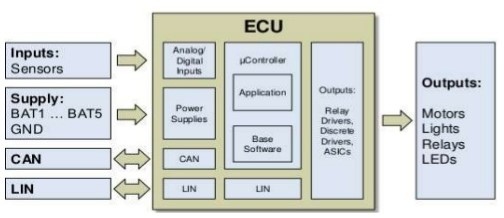
\includegraphics[width=\linewidth]{images_folder/electronic-control-unitecu-6-638.jpg}
    \caption{ECU structure}
    \label{fig:ECUHW}
\end{figure}
The hardware structure of an ECU is composed by complex series of components, to better understand the overall organization, without entering in to much of a engineering detail a block scheme overview is offered by \ref{fig:ECUHW}.\\
It´s possible to easily differentiate between four different parts:
\begin{itemize}
    \item Power supply, handle the power input for the board and for the power components such as the motor driver or other power electronics components needed to drive the controlled parts. 
    \item Inputs, which can be either analog and digital inputs
    \item Communications link, such as CAN and LIN.
    \item Outputs, the output are mainly composed by mechanical components that require electrical actuation in order to perform engine required tasks. Other output that can be found are related to the sharing of information with other ECUs.
    \item MPU, Microprocessor unit and memory, in general Flash and RAM. 
\end{itemize}
\subsection{CAN - Communication protocols in ECU}
The Controll Area Network (CAN) is a serial communication protocol suited for networking sensors, actuators and other node in real-time systems. The CAN specifications define the protocols only for the physical layers and the data link layers. These layers are part of the OSI, Open System Interconnections, an abstraction model for communication protocol. 
\begin{figure}[h]
    \centering
\begin{tikzpicture}[box/.style={on chain,join,draw,minimum width=4cm,minimum height=1cm,
align=center},start chain=going below, node distance=5mm,font=\sffamily,fbox/.style={draw,thick,fill=white}]
  \node[box] (a) {Application layer};
  \node[box] (b) {Presentation layer};
  \node[box] (c) {Session layer};
  \node[box] (d) {Transport layer};
  \node[box] (e) {Network layer};
  \node[box] (f) {Data Link layer};
  \node[box] (g) {Physical layer};
  \node[above=1cm, xshift=1mm] (l) {Application A};
  \begin{scope}[on background layer]
   \node[fbox,fit=(a|-l.north) (g),inner xsep=3mm] (f1){};
  \end{scope}
\end{tikzpicture}
    \caption{OSI}
    \label{fig:ECUstructure}
\end{figure}
The OSI is an abstraction model for the communications protocols. The main layer that are needed to be analyzed are the physical layer and the Data link layer. Just for reference purpose the top upper layer, the application layer defines what to do with the data received in the physical layer.\\
The physical layer is indeed composed by the physical transport media, form cables to the plug and sockets. CAN use a twisted pair in which the differential voltage between the couple is used to represent the bits transmitted. The Data link layer defines the MAC, Media Access Control Methods. In CAN this is set to CSMA/CA or Carrier Sense Multiple Access/ Collision Avoidance. What this complex series of acronyms stand for is that in CAN on the bus a message can be sent only if the bus is free, in case two nodes send a message contemporaneously, then the message with the highest priority win and the node with the low priority message retrieve to a receiver status.
\subsubsection{CAN message format}
\begin{figure}[h]
    \centering
    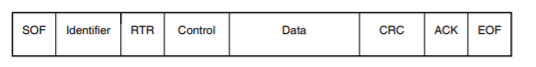
\includegraphics[width=\linewidth]{images_folder/can message.png}
    \caption{CAN message structure}
    \label{fig:CANMSG}
\end{figure}
CAN distinguish different message formats, in here it´s analyzed only the data frame format. The data frame consist essentially of:
\begin{itemize}
    \item SOF, start-of-frame, which denotes the start of the transmission. The length is 1 bit. 
    \item Identifier, the 11 bit identifier is used not only to identify the message but to define its priority. 
    \item RTR, remote transmission request, define the difference between a message sent and a remote request. 
    \item Control bits, consist of 6 bits and define how many bites of data follow in the data field. In theory not all of the 6 control bits are used to identify the length of the data, since this one is limited to a maximum of 8 bytes. With that being said the actual number of bits reserved to define the data length is 4, which is a bit more than necessary. This is done to allow controller to send data which is more than 8 bytes (9 - 15) in special cases.
    \item Data, actual data to be sent, with a maximum of 8 bytes ($64$ bits = maximum value that can be sent is $2^64 - 1$).
    \item CRC, cyclic redundancy checks, enable the receiver to chunk if the received bits have been corrupted. The techniques used are bit monitoring and bit stuffing.
    \item ACK, consist of a two bit acknowledgement used by the transmitter to receive an acknowledgment of validity form the receiver.
    \item EOF, end-of-frame, is a seven bit signal that define the end of communications. 
\end{itemize}
\subsubsection{CAN arbitration}
Arbitration is the mechanism that handle bus access conflict. As already underlined when describing the can Data link layer, based on collision avoidance every node can start sending if the bus is free, in the eventuality in which two nodes start the communication simultaneously arbitration comes into place, solving the conflict. During the arbitration phase each transmitting node send the identifier and compares it with the other by motoring the level of the bus. Whenever a node sense a dominant level on the bus, while sending a recessive one, than the node stop the communications and become a receiver. In CAN a recessive level is couple with the bit 1, while a dominant with 0. Consider having three nodes with the following identifiers:
\begin{equation}
I_{1} = 11001101010
\end{equation}
\begin{equation}
I_{2} = 11001011011
\end{equation}
\begin{equation}
I_{3} = 11001011001
\end{equation}
\begin{figure}[h]
    \centering
    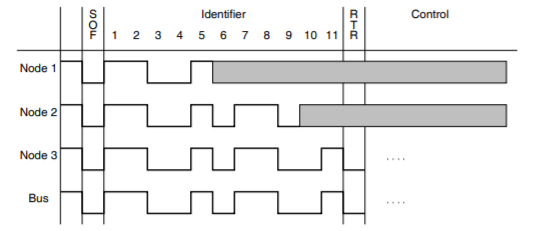
\includegraphics[width=\linewidth]{images_folder/can_arbitration.png}
    \caption{CAN arbitration}
    \label{fig:CANABR}
\end{figure}
As exemplified in \ref{fig:CANABR} the nodes starts by sending the SOF, then the identifier comes into play. The nodes continue to send their identifier until all are equal to each other. At bit number 6  the $I_1$ set the bus on a recessive level while sensing both from $I_2$ and $I_3$ a dominant level, therefor $I_1$ stop the communication and switch to a receiver mode. Since the tenth bit of $I_2$ is at recessive level while $I_3$ is at dominant. Node $I_3$ is the transmitter and therefor continue with the transmission of the other part of the data frame. CAN is affected by starvation´s problems. Low priority nodes may expect large latency in case of high priority units being very active. \\
It´s important to underline the fact that there is no message destination address in CAN, instead each node picks up all the traffic on the bus.\\
In order to better understand the can arbitration mechanism consider the following example in which the can nodes are exemplified by open collector transistors. 
The level of the bus is at a low level (dominant) in case any number of transistor in the network output a dominant level (that is why zero is dominant, only one transistor is closed an the whole bus sees a zero on it). The bus will only be at high level (recessive) when all the transistors in the network output a recessive level (the transistors are open, putting a 1 on the bus).
\begin{figure}[h]
    \centering
    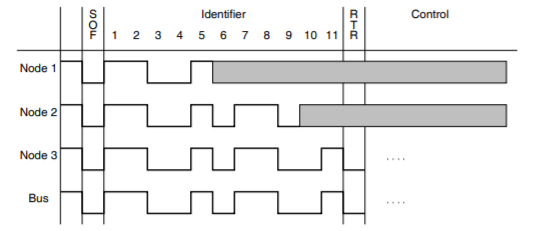
\includegraphics[width=\linewidth]{images_folder/can_arbitration.png}
    \caption{CAN arbitration}
    \label{fig:CANABR}
\end{figure}
\section{AUTOSAR}
AUTomotive Open System ARchitecture (AUTOSAR) is an open and standardize automotive software architecture, jointly develop by automobile manufacturers, supplier and tool developer. AUTOSAR architecture was introduced to promote standardization of the software development process of Automotive Electronic Control Units (German: Steuergerät). Prior to the introduction of Autosar ECU software needed to be completely fitted around the components architecture, decreasing to close to zero the portability over different ECU platforms and between different producer. 
AUTOSAR introduced a layer in between the software and the hardware that ensures that the developed application is completely independent from the hardware platform. 
\begin{figure}[h]
    \centering
    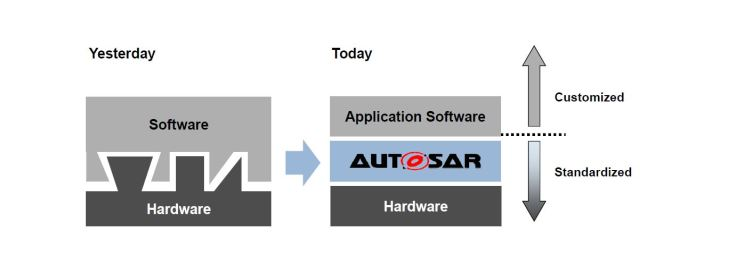
\includegraphics[width=\linewidth]{images_folder/autosarcapture.jpg}
    \caption{Autosar interface}
    \label{fig:AUTCA}
\end{figure}
\subsection{AUTOSAR Architecture}
The architectural structure of the AUTOSAR standard is used to divide the hardware-independent software and the hardware-oriented software. Three main layers can be identified:
\begin{itemize}
    \item Application software, host all the functions that control the vehicle capabilities. In the AUTOSAR language functions are also called SWC (software components). An example of functions could be the software driving the windshield wipers. These software need to be able to receive a switch input in order to activate and give an output to light up the relative led on the dashboard. 
    \item Basic Software (BSW), includes low level software like services and hardware specific software. Related to the previous example this gives the input output functionality required by the windshield wipers function. 
    \item Run-time Environment (RTE), abstraction layer that manage the interface between the tow other layers. 
    \item Virtual Functional Bus (VFB), this is an additional architectural strategy introduced by autosar to decouple applications (windshield wiping) from the hardware infrastructure. The virtual bus map the two main type of communication between SWCs (intra-ECU and inter-ECUs) to the same function, allowing the user to simply define a communication, without having to bother about the protocol required (inter-ECUs is generally based on CAN while intra uses shared memory). The connection mapping is implemented by the RTE and becomes the concrete interface between individuals SWCs and between SWCs and the BSW.
\end{itemize}
\begin{figure}[h]
    \centering
    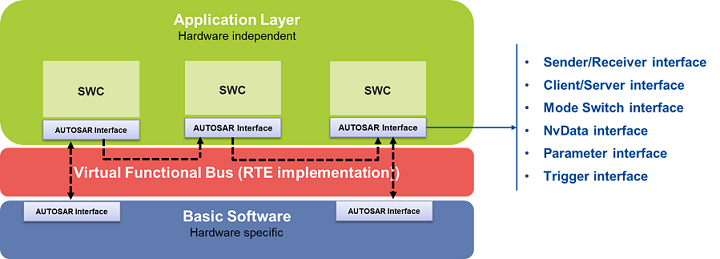
\includegraphics[width=\linewidth]{images_folder/878x-autosar_layers.b68.png}
    \caption{Autosar layers}
    \label{fig:AUTLAY}
\end{figure}
\subsection{Application Software Layer}
The application layer consist of the various software components interacting together. 
To connect software components, each component has well defined ports through which the component can communicate with other components or with Basic Software modules. The autosar architecture defines 2 types of software components:
\begin{itemize}
    \item Application SWC, implement an application. This SWC type can use all the AUTOSAR communication mechanism but can communicate to the sensors only via a Sensor-Actuator type software component. 
    \item Sensor-Actuator type SWC, has access to ECU specific hardware I/O signals. This SWC is responsible for reading a sensor and provide its data to other components or to set the status of an actuator. 
\end{itemize}
The SWC communicates via Ports. A port is used to send or request information. Once a port is definited it needs to be associated with the interface that define the information exchange. The main interaces that can are supplied by AUTOSAR are the following:
\begin{itemize}
    \item Sender/Receiver, defines a set of data elements that are sent from one components to another. 
    \item Client/Server, a server can implement a set of operation and make the result available to the clients. This work as a function call for the clients. 
    \item Parameter interface, define a set of parameters (constant or calibrate)
    \item Non-volatile data access, provides access to Non volatile data. 
    \item Trigger interface, give a SWC the ability to trigger another SWC. This works as an interrupt. 
    \item Mode-Switch, activate particular modes of use. 
\end{itemize}
\subsection{SWC structure - AUTOSAR Internal Behaviour}
Every SWC is not just composed by runnable code, in order to withstand the AUTOSAR standar a certain architecture need to beimplemtned in every SWC. The main IB elements of an SWC are the following:
\begin{itemize}
    \item Runnables, these are the pieces of code which implement the SWC functionality. A single SWC can have multiple runnables. 
    \item RTE-Event, in real time environment such as the ECU the scheduling information of an SWC, its priority and frequency of execution need to be defined. Those can be found inside the RTE-Events. 
    \item Access Point, the access point specify how each runnable expect to access the information conveyed through the SWC connection interfaces. 
\end{itemize}
\subsection{Example implementation of a windshild wiper control}
Having defined the AUTOSAR standard structure, it´s useful to define an example of implementation to better understand. Consider the function windshield wiping. The function graphical structure can be defined as follows:
\begin{figure}[H]
    \centering
    \includegraphics[width=\linewidth]{images_folder/{AE149F77-9676-4E55-B728-C6B8FD1F5218}.png}
    \caption{Windshield wipers implementation}
    \label{fig:WINWIP}
\end{figure}
The contains tree instances of the Sensor-Actuator SWC. The first is the sensor reading the status of the windshield wiper switch, the read is done via the IO labeled port. The status is transmitted via a service. The other sensor instead check the status of the vehicle, on weather or not this is on or off. The transmission is done via a sender receiver. The main difference between the two is that the server/client configuration that the data from a server is only available to the client requesting the data. On the other hand a receiver/sender configuration the data is "published" on the RTE, and the connected receiver/writer can access/modify the data.\\
The only actuator SWC is the one in charge of controlling the windwipers motor. The managing component is the one who compile the logic of the acutaion. It is client of the Swithc, and can therfore request the status (the request periodicity is defined by it´s RTE event element). Based on it and on the information from \textit{Car status} define an actuation that is given as service to the client \textit{Actuator Windschield}. The managging components also have a Nvblock which allow it to save its interanl state to the non volatile memory. 
The design can be done aoviding entering inECU specific details. To create a real application two more steps are required. The first one is to define the manging block behaviour through an executable and the second one is the passage from VFB commnication to real ECU. This is done by the runtime einvoroamnte 

\section{Model based design}
\subsection{Introduction}
Inside the automotive world the trend that has drawn more differences in the way car are constructed is in the electronic components side. if the cost related to the development of mechanical components, safety features and logistic increased constantly through the years, the cost related to the electronic components exponentially increased. What once was a mechanical system is most probably going to be a embedded system nowadays. The increase in hardware related to embedded components requires an increase in the software in order to control it. The yearly increase in lines of code for car is a statement in support of the importance of software. 
\begin{figure}[H]
    \centering
    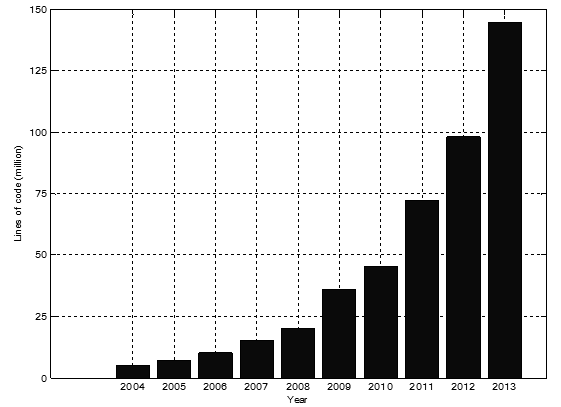
\includegraphics[width=\linewidth]{images_folder/Yearly-increase-in-automotive-software-complexity-shown-by-million-lines-of-code-of-1-ConvertImage.png}
    \caption{Yearly increase in automotive software complexity}
    \label{fig:yearlyincreas}
\end{figure}
Software development therefor faces new challenges, related to shorten development time, a high need of scalability  not only in the software but also in the development platforms, complex safety requirements and adaptability over continuously changing hardware.\\
Model based design has entered the automotive conversation because it can full fill the previously reported challenges. The model based approach brings two main characteristic to the table: on the one hand it gives a development platform which is component independent, therefor allowing for better integration through rapidly changing hardware, on the other hand makes the integration of new features not time depended. In this sense it recall a concept similar to Scurm, where changes are welcomed during the whole development process. in this case, with model based design, changes are welcomed during the whole life of the software.
\subsection{Model based design}
Model-Based Design provides a mathematical and visual approach to develop complex control and signal processing systems. It centers on the use of system models throughout the development process for design, analysis, simulation, automatic code generation and verification \cite{Mathworks}. The main features are abstraction and automation. As reported by \cite{modelbased} model based tackle complexity via abstraction and automation. Abstraction is achieved by the using suitable models of a software system, while automation is achieved by systematically transform these models into executable source code.\\
Engineers create a model to specify the behavior of an embedded system; the model, which consists of block diagrams, textual programs, and other graphical elements, is an executable specification that lets engineers run simulations to test ideas and verify designs throughout the development process. The main advantages are
\begin{itemize}
    \item The design can be tested, refined and retested throughout the development process, thus increasing product quality. Test and validation are done continuously rather than at the end of the process. Error can be found before hardware is required for testing
    \item Simplification of complex system, by providing a graphical design models simplify the creation of high complexity functions, especially when compared with hand code components. This advantage as it enhance and simplify communication inside the team, as it is easy to understand the models. 
    \item Embedded code can be generate automatically from the models. To adapt the model to different hardware there´s the need to adjust the compiler, not every single model. This allow for great adaptability to rapidly changing hardware. 
\end{itemize}

\cleardoublepage
\end{document}
